\chapter{Segmento terrestre} \label{tierra}
\minitoc

Para asegurar el cumplimiento de los objetivos de la misión, resulta imprescindible disponer de una estación de comunicaciones capaz de recibir los datos generados por la constelación. El segmento Tierra comprende el conjunto de infraestructuras y recursos ubicados en la superficie terrestre dedicados a la gestión, control y operación de los sistemas espaciales. Su función no se limita únicamente a la recepción de información, sino que abarca también tareas de telemetría, seguimiento, control, envío de comandos y mantenimiento orbital. En este apartado se presenta un análisis conciso del segmento terrestre, con el propósito de validar la viabilidad técnica de la misión propuesta.
\newpage
\section{Elección del emplazamiento}

Primeramente, se evaluan las posibles opciones de estaciones terrestres que puedan utilizarse para la presente misión. Dichas opciónes son:


\begin{enumerate}
    \item \textbf{Estación de Fairbanks, Alaska (NOAA)}: Ubicada en Gilmore Valley, esta estación es la instalación de comunicaciones satelitales más septentrional de Norteamérica, recibiendo más datos ambientales que cualquier otra estación.
    \item \textbf{Estación de Wallops, Virginia}: La estación de Wallops constituye otra instalación fundamental de NOAA para adquisición de datos satelitales, localizada en Wallops Island a 37.94°N, -75.47°W . Esta estación opera como parte del Wallops Flight Facility y proporciona capacidades especializadas para satélites de observación terrestre . La instalación funciona como sistema de respaldo para la estación primaria de Fairbanks . El complejo incluye sistemas de comunicación por satélite geoestacionarios y facilidades para procesamiento de datos \cite{noaa_wallops_2019}.
    \item \textbf{Red de Estaciones Europeas}: EUMETSAT opera una red de estaciones terrestres europeas desde su centro de control en Darmstadt, Alemania (49.87°N, 8.65°E) . Las estaciones principales incluyen Fucino, Italia (41.98°N, 13.60°E) y Cheia, Rumania . La estación de Svalbard, Noruega (78.23°N, 15.41°E) proporciona servicios para satélites de órbita polar  \cite{eumetsat_ground_segment_2025}.
    \item \textbf{Implementación de una estación propia}: Opción que requeriría mayor inversión inicial pero podría personalizarse específicamente para nuestra misión.
\end{enumerate}

\begin{figure}[H]
    \centering
    \includegraphics[width=.5\linewidth]{7.Segmento_Tierra/AS3_oct-4-2022-1-scaled.png}
    \caption{Antena de banda X de la estación de Fairbanks, Alaska. \\
    Fuente: \cite{ASF2025_NSN}.}
\end{figure}

Tras exponer estas opciones, \textbf{la Estación de Fairbanks, Alaska}, emerge como la opción idónea. Esto se fundamenta en su ubicación geográfica óptima, situada a una latitud elevada (64.9°N), lo que posibilita numerosos contactos diarios con satélites en órbitas cuasi-polares, maximizando el tiempo de descarga. La estación cuenta con infraestructura necesaria, integrada por antenas de 26 metros y varias de 13 metros, todas ellas con capacidad en banda X, requeridas para esta misión. Además, la estación de Fairbanks actúa como nodo central de la Red Ártica de Comunicaciones Satelitales, interconectada con otras estaciones de alta latitud, como ESTRACK (ESA), con estaciones en Svalbard (Noruega) y Kiruna (Suecia); y  Near Space Network (NASA) con enlaces a Wallops (Virginia) y McMurdo (Antártida) \cite{noaa_fairbanks_2023}.

\section{Descarga de los datos generados. Viabilidad.}

Para validar la elección del emplazamiento, se realiza una simulación en MATLAB cuya función sera analizar el tiempo de contacto semanal de los satélites con la estación de Tierra. Para ello, se implementará un escenario de Aerospace Toolbox. 
Primeramente se establecen los parámetros temporales de la simulación, definiendo una semana de observación con un muestreo de un minuto. Se especifica la localización de la estación de Tierra (64,84º, -147,712º) y una elevación mínima de contacto $\epsilon = 10º$, así como las características orbitales de la constelación. Con ello, se determina el conjunto de intervalos de acceso, es decir, los periodos en los que existe visibilidad suficiente (elevación mayor al umbral) para la transmisión de datos hacia la estación de Tierra. El resultado, a lo largo de una semana, es de \textbf{79620 segundos, o 22,12 h para la constelación}.

\begin{figure}[H]
    \centering
    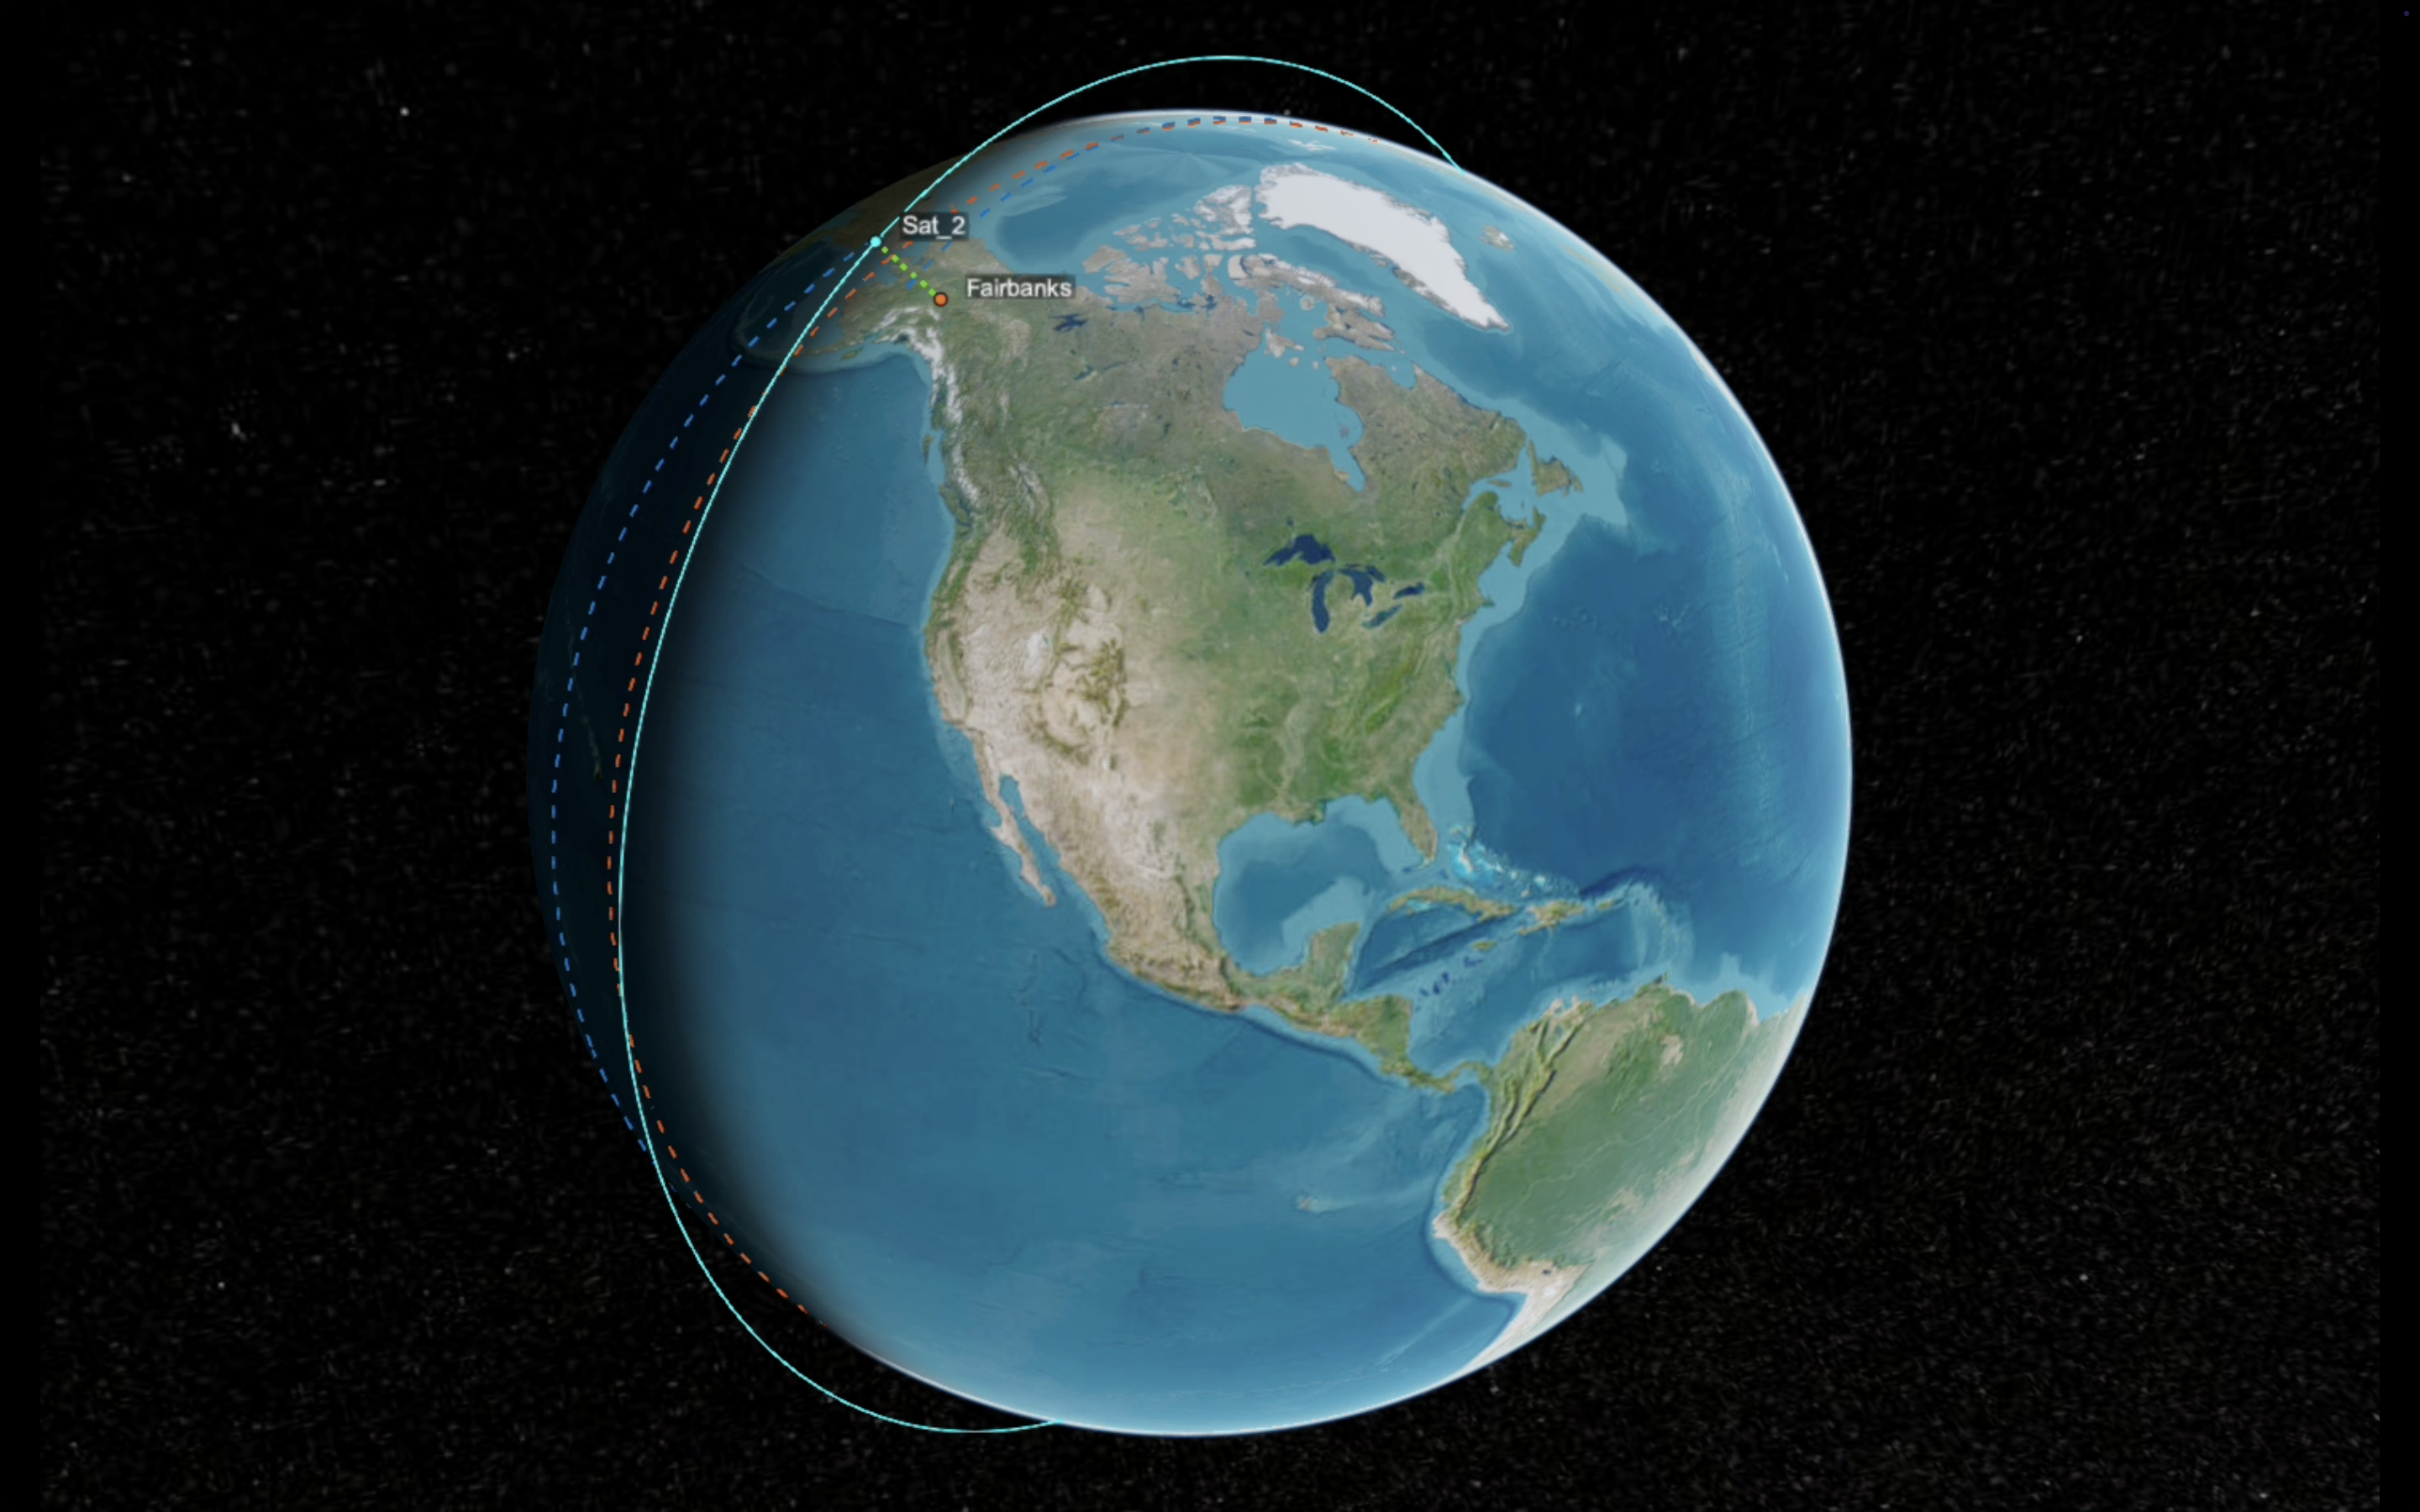
\includegraphics[width=1\linewidth]{7.Segmento_Tierra/analisis_contacto.jpg}
    \caption{Escenario de simulación creado con \textit{Aerospace Toobox}. \\Fuente: Elaboración Propia}
\end{figure}

\begin{figure}[H]
    \centering
    \begin{subfigure}[b]{0.3\textwidth}
        \centering
        \includegraphics[width=\textwidth]{7.Segmento_Tierra/Traza 2D 1 Orbita.jpg}
        \caption{Traza en 1 órbita completa }
        \label{fig:traza1}
    \end{subfigure}
    \hfill
    \begin{subfigure}[b]{0.3\textwidth}
        \centering
        \includegraphics[width=\textwidth]{7.Segmento_Tierra/Traza 2D 1 Dia.jpg}
        \caption{Traza en 1 día}
        \label{fig:traza2}
    \end{subfigure}
    \hfill
    \begin{subfigure}[b]{0.3\textwidth}
        \centering
        \includegraphics[width=\textwidth]{7.Segmento_Tierra/Traza 2D 1 Semana.jpg}
        \caption{Traza semanal}
        \label{fig:traza3}
    \end{subfigure}
    \caption{\textit{Ground tracks} sobre la región de interés. En rojo: Estación de Fairbanks \\ Fuente: Elaboración propia}
    \label{fig:conjunta}
\end{figure}


\subsection{Velocidad de descarga}\label{sec:downlink}



El transmisor de banda X permite velocidades de descarga teóricas de hasta 150 Mbps, según especificaciones del fabricante. Esto se produce en condiciones óptimas, pero diversos factores ambientales y operativos reducen este valor en la práctica.

\subsubsection{Atenuamiento por inclemencias meteorológicas}

Las gotas de agua y cristales de hielo dispersan y absorben las ondas electromagnéticas, reduciendo la intensidad de la señal que llega a la estación terrestre. Este efecto es más pronunciado en frecuencias más altas como la banda X, donde las longitudes de onda son comparables al tamaño de las gotas. Primeramente se plantean las velocidades que esperables en función de la inclemencia meteorológica de un día cualquiera:

\begin{table}[H]
\centering
\caption{Velocidades de transmisión aproximadas en función de las condiciones meteorológicas. \\ Fuente:\cite{rain_attenuation_xband_2012}.}
\begin{tabular}{ll}
\hline
\textbf{Condición Meteorológica} & \textbf{Velocidades (Mbps)} \\
\hline
Cielo despejado & 120 - 150 \\
Lluvia moderada & 75 - 100 \\
Tormenta extrema & 22 - 38 \\
Nubes densas & 90 - 110 \\
\hline
\end{tabular}

\end{table}

Se debe considerar la estacionalidad a lo largo del año, teniendo en cuenta por ejemplo, que el verano de Alaska es mas lluvioso que el invierno. Con ello, se puede representar gráficamente las velocidades que  esperables a lo largo del año, así como sacar una velocidad media anual. Tomando las siguientes probabilidades:

\begin{table}[H]
\caption{Distribución estacional de condiciones meteorológicas en Fairbanks. \\Fuente: \cite{climate_data_fairbanks}.}
\centering
\begin{tabularx}{\textwidth}{X X X X X}
\toprule
\textbf{Estación} & \textbf{Cielo despejado (\%)} & \textbf{Lluvia moderada (\%)} & \textbf{Tormentas extremas (\%)} & \textbf{Nubes densas (\%)} \\
\midrule
Invierno  & 80 & 15 & 1  & 4  \\
Primavera & 65 & 25 & 5  & 5  \\
Verano    & 55 & 30 & 10 & 5  \\
Otoño     & 70 & 20 & 5  & 5  \\
\bottomrule
\end{tabularx}

\end{table}

Se modela la simulación en MATLAB y representando gráficamente se extrae:

\begin{figure}[H]
    \centering
    \includegraphics[width=1\linewidth]{7.Segmento_Tierra/velmediasemanal.png}
    \caption{Velocidad de descarga de datos semanal a lo largo de 1 año. \\Fuente: Elaboración Propia}
\end{figure}

\begin{figure}[H]
    \centering
    \includegraphics[width=1\linewidth]{7.Segmento_Tierra/veldiariabandax.png}
    \caption{Velocidad de descarga diaria estimada en función de condiciones climáticas.\\ Fuente: Elaboración Propia}
\end{figure}

Se aprecia una velocidad media anual de \textbf{116,8 Mbps}, lo cual supone una pérdida del 22,13\% debido a las condiciones climáticas.


\textbf{Otros factores correctores.}

De este ultimo valor, se aplican dos factores correctores adicionales:
\begin{itemize}
    \item \textbf{Factor corrector por hardware}: El hardware introduce una reducción del \textbf{12.5\%} en la velocidad debido a pérdidas en componentes como antenas, cables y receptores. Las antenas tienen una eficiencia operativa del 65-70\%, lo que genera pérdidas inherentes en la captación y transmisión de la señal. Además, factores como desadaptación de impedancia (~1 dB) y ruido térmico (~0.5 dB) contribuyen a esta disminución \cite{altunc_xband_cubesat_2016}.
    \item \textbf{Factor corrector por paso baja elevación}:
    Los pases de baja elevación (\textless 30°) afectan la velocidad debido a la mayor distancia que debe atravesar la señal y su exposición prolongada a interferencias atmosféricas. Esto genera un aumento significativo en la atenuación y reduce los tiempos de contacto efectivos. Este factor introduce una reducción adicional del \textbf{25\% \cite{satellite_coordinates_look_angles}}.
\end{itemize}

Por lo que la velocidad de transmisión de datos real será:
$$
\text{Velocidad real} = 116\ \text{Mbps} \times 0.875 \times 0.75 = \boxed{76.1\ \text{Mbps}}
$$

Existen otros fenómenos que pueden hacer fluctuar la velocidad real de descarga. Sin embargo, en este trabajo solo se han considerado los de mayor peso.

\subsection{Generación de datos. Viabilidad de la estación. Memoria de a bordo}

Una vez evaluada la velocidad de descarga, se debe conocer también el volumen de datos generados que la constelación captura todas las semanas. Asumiendo los siguientes parámetros:

\begin{itemize}
\item Número de bandas espectrales: $N_{\text{bandas}} = 3$
\item Resolución espacial (GSD): $80$ metros
\item Área a mapear (EE. UU. continental): $9.826.675$ km$^2$ (Fuente: \cite{cia_worldfactbook_usa_area})
\item Bits por banda: $12$ bits
\end{itemize}

El volumen de datos se calcula mediante la ecuación:

\begin{equation}
\text{Volumen de datos} = \frac{N_{\text{bandas}} \times \text{bitsPerBand} \times \text{Area}_{\text{Map}} \times 10^6}{\text{GSD}^2 \times 8 \times 10^9}
\end{equation}

Sustituyendo los valores:
\begin{equation}
\text{Volumen de datos (GB)} = \frac{3 \times 12 \times 9.826.675 \times 10^6}{80^2 \times 8 \times 10^9} = \boxed{6{,}909\ \text{GB}}
\end{equation}

\subsubsection{Viabilidad de la estación}

Por último, una vez calculados estos factores, resulta sencillo evaluar la viabilidad del sistema en función de la capacidad de descarga de la estación de Tierra. El tiempo mínimo necesario para transferir todos los datos generados durante la semana es:
\begin{equation}
t_{\text{descarga}} = \frac{6,909\ \text{GB}}{76,1\ \text{Mbps} \times \frac{1}{8}\ \text{MBps}} = \frac{5681,6}{9,5} = 727\ \text{segundos}
\end{equation}

Teniendo en cuenta que el tiempo total de contacto disponible entre el satélite y la estación de Tierra durante ese mismo periodo es, calculado previamente, es  $t_{\text{contacto, semana}} = 79620\ \text{segundos}$, se verifica que $t_{\text{descarga}} < t_{\text{contacto, semana}}$. Por tanto, la configuración propuesta es viable desde el punto de vista de la capacidad de descarga, ya que existe un margen más que suficiente para completar la transferencia incluso considerando posibles interrupciones o ineficiencias del enlace.

\subsubsection{Gestión de la memoria de a bordo}

Por último, se modela el estado de la memoria de cada satélite a lo largo del tiempo, considerando tanto la generación continua de datos como la descarga durante los accesos, verificando que la memoria no se sature. En caso de que algún satélite agote su capacidad de almacenamiento, se considera que la configuración no es viable. Mediante el escenario de \textit{Aerospace Toolbox} creado previamente, y utilizando la velocidad media de descarga calculada en el apartado \ref{sec:downlink}:

\begin{figure}[H]
    \centering
    \includegraphics[width=1\linewidth]{7.Segmento_Tierra/memoria.jpg}
    \caption{Evolución de la memoria a bordo de los satélites a lo largo de 1 semana.\\ Fuente: Elaboración Propia}
\end{figure}

Se observa que, aunque existen periodos donde los satélites no tienen contacto con la estación durante varias horas, una memoria de apenas 512MB es más que suficiente para almacenar estos datos. Sería interesante aumentar este límite a 1GB o incluso más. Las tecnologías actuales de discos de estado sólido SSD permiten almacenamientos muy superiores a este sin una penalización significativa del peso. Esto permitiría almacenar los datos en el caso de pérdidas de conexión temporales o periodos de mantenimiento en la estación de Tierra, dando así una mayor robustez a la misión.